\PassOptionsToPackage{unicode=true}{hyperref} % options for packages loaded elsewhere
\PassOptionsToPackage{hyphens}{url}

\documentclass[9pt]{beamer}

\usepackage[french]{babel}

%\usetheme{hsrm}
%------------------------------
\useinnertheme[shadow=true]{rounded}
\useoutertheme{infolines}

%\setbeamerfont{block title}{size={}}
\definecolor{bleulapis}{HTML}{247BA0}
\definecolor{rouge}{HTML}{A41D22}
\definecolor{noire}{HTML}{262626}

\setbeamercolor{alerted text}{fg=rouge}
\setbeamercolor*{palette primary}{fg=white,bg=white!30!bleulapis}
\setbeamercolor*{palette secondary}{fg=white,bg=white!40!bleulapis}
\setbeamercolor*{palette tertiary}{fg=white,bg=white!50!bleulapis}
%\setbeamercolor*{palette quaternary}{fg=darkblue,bg=yellow!20!orange}

\setbeamercolor*{sidebar}{fg=bleulapis,bg=white}
\setbeamercolor{block title}{bg=bleulapis,fg=white}
%\setbeamercolor*{palette sidebar primary}{fg=darkblue!10!black}
%\setbeamercolor*{palette sidebar secondary}{fg=white}
%\setbeamercolor*{palette sidebar tertiary}{fg=darkblue!50!black}
%\setbeamercolor*{palette sidebar quaternary}{fg=yellow!10!orange}

\setbeamercolor*{titlelike}{parent=palette primary}
\setbeamercolor{frametitle}{fg=white,bg=bleulapis}
%\setbeamercolor{frametitle right}{bg=yellow!60!orange}

\setbeamercolor*{separation line}{}
\setbeamercolor*{fine separation line}{}
\setbeamertemplate{enumerate items}[default]
\setbeamertemplate{itemize items}[default]
%\setbeamercolor{palette tertiary}{fg=white, bg=blue}
\usepackage{tikz}
\usepackage[tikz]{bclogo}
\usetikzlibrary{positioning}
\usetikzlibrary{mindmap,backgrounds,shapes,decorations}
\usepackage{wrapfig}
\usepackage{minted,listings}


\usepackage{hyperref}
\usepackage{array}
\makeatletter
%%%%%%%%%%%%%%%%%%%%%%%%%%%%%% Textclass specific LaTeX commands.



\usepackage{pifont}
\usepackage[tikz]{bclogo}
\usetikzlibrary{positioning}
\usepackage{wrapfig}
\usepackage{mathrsfs}
\usetikzlibrary{arrows}
\usepackage{multicol}

\usepackage{hyperref}
\hypersetup{
            pdftitle={Les Signaux},
            pdfauthor={Pascal Malingrey},
            pdfkeywords={NSI, Signaux, Linux},
            pdfborder={0 0 0},
            breaklinks=true}
\urlstyle{same}  % don't use monospace font for urls
\usepackage{xcolor}
\usepackage[tikz]{bclogo}
\usepackage{wrapfig}
\usepackage{framed}
\usepackage{algorithm}
\usepackage{algpseudocode}%MISE EN PAGE

\definecolor{codegreen}{rgb}{0.1,0.47,0.1}
%initial : {0,0.6,0}
%\definecolor{codeblue}{rgb}
%20, 148, 20)
\definecolor{fondjaune}{rgb}{0.99, 0.7,0.8}
%255, 255, 153)
%254, 191, 210
\definecolor{couleurdef}{rgb}{0.99, 0.8, 0.87}
\definecolor{codegray}{rgb}{0.5,0.5,0.5}
\definecolor{codepurple}{rgb}{0.58,0,0.82}
\definecolor{backcolour}{rgb}{0.95,0.95,0.92}

\newenvironment{code}[1]{%
    \begin{bclogo}[couleur=backcolour, couleurTexte=black ,couleurBord=bleulapis ,couleurBarre=black, ombre=false,epBord=0.9,logo=\#,arrondi=0.1]{{\bfseries #1}}%
    }%
    {%
    \end{bclogo}
}%

\setbeamertemplate{theorems}[numbered]
\newtheorem{exercise}{Exercice}

\usepackage{minted}
\title{Les Signaux}
\subtitle{Version 1}
\author{Pascal Malingrey}
\institute{Académie Strasbourg}
\begin{document}
\maketitle

\section{Première approche}

\defverbatim \exe{
\begin{minted}{bash}
nsi@lin$ python3 ex1.py
\end{minted}
}

%---------------------------- FRAME-------------------------------------------
\begin{frame}{STOP ou ENCORE}
Vous disposez dans votre dossier d'un fichier \textbf{ex1.py} (son contenu n'a pas d'importance pour le moment.)
Dans un terminal vous exécuter la commande suivante:

\begin{code}{terminal}
 \parbox{6cm}{\exe}
\end{code}

\begin{enumerate}[<+->]
\item Que constatez vous ?
\item Comment interrompre le programme , tout en gardant le terminal actif?
\item On va appuyer sur une combinaison de touche \texttt{Ctrl+C}
\end{enumerate}

\end{frame}
%---------------------------- FRAME-------------------------------------------

\begin{frame}{Que s'est-il passé?}

La combinaison de touche \texttt{Ctrl+C} a interrompu l' exécution du programme.
Cela signifie deux choses:

\begin{itemize}
\item ``quelque chose'' est à l'écoute du clavier
\item le programme traite l'information de la combinaison \texttt{Ctrl+C}
\end{itemize}

\end{frame}
\section{Deuxième approche}

%---------------------------- FRAME-------------------------------------------
    
  \begin{frame}{Commande shell}

La commande \texttt{cat} est utilisée qu'à titre d'exemple, sa
fonctionnalité n'est pas importante ici. Par contre les suivantes sont
utiles:

\begin{itemize}
\item \texttt{ps} : liste les processus dans le terminal
\item \texttt{\^{}z} : Ctrl+z suspend un processus
\item \texttt{fg} : reprend un processus
\end{itemize}

\end{frame}

%---------------------------- FRAME-------------------------------------------

\defverbatim \exun{
\begin{minted}{bash}
nsi@lin$ cat
nsi@lin$ ^z  #Appui Ctrl+z
nsi@lin$ ps
\end{minted}
}
\defverbatim \exdeux{
\begin{minted}{bash}
PID TTY          TIME CMD
25280 pts/0    00:00:00 bash
26623 pts/0    00:00:00 cat
26624 pts/0    00:00:00 ps
\end{minted}
}
  \begin{frame}{Dans un terminal}
\begin{columns}
    \begin{column}{0.5\textwidth}
   
        \onslide<1->
        Les commandes
       
                 \begin{code}{terminal}
                     \parbox{6cm}{ \exun}
           \end{code}
    \end{column}

    
    \begin{column}{0.5\textwidth}  
                \onslide<2->
        Le résultat
        
       \begin{code}{terminal}
             \parbox{6cm}{  \exdeux}
       \end{code}
    \end{column}
\end{columns}

\onslide<3->

On voit trois processus \begin{itemize}
    \item le bash (qui correspond à notre terminal)
    \item cat (qu'on a lancé)
    \item  ps (qui liste nos processus)
\end{itemize} 

Remarque : Vous constatez que les numéros de PID ne sont pas les mêmes chez vous.
\end{frame}
%---------------------------- FRAME-------------------------------------------

\defverbatim[colored] \exun{
    \begin{minted}[autogobble]{bash}
nsi@lin$ killall -2 cat
nsi@lin$ ps
    \end{minted}
}
\defverbatim [colored]\extrois{
    \begin{minted}{bash}
     nsi@lin$ ps
    \end{minted}
}

\begin{frame}{Stoppons le processus cat}

Nous allons envoyer un signal de terminaison (comparable au Ctrl-C) au processus \textbf{cat} par le biais de la commande \textbf{killall}. killall  envoie un signal aux processus dont le nom est indiqué avec le numéro du signal.\\
Regardons ce qu'il en est des processus

\begin{columns}
    \begin{column}{0.5\textwidth}

        \onslide<1->
        Les commandes
        
        \begin{code}{terminal}         
          \parbox{6cm}{  \exun}
        \end{code}
    \end{column}
    
    
    \begin{column}{0.5\textwidth}  
        \onslide<2->
        Le résultat
        
        \begin{code}{terminal}
           \parbox{6cm}{ \exdeux}
        \end{code}
    \end{column}
\end{columns}


\alert{\large Aucune différence !!}

\end{frame}

%---------------------------- FRAME ------------------------------------------

\defverbatim[colored] \exun{
    \begin{minted}[autogobble]{bash}
    nsi@lin$ fg
    nsi@lin$ ps
    \end{minted}
}
\defverbatim[colored] \exdeux{
    \begin{minted}[autogobble]{bash}
    PID TTY        TIME CMD
    25280 pts/0   00:00:00 bash
    26624 pts/0   00:00:00 ps
    \end{minted}
}

\begin{frame}{ Reprise du processus}

 On va demander une reprise du processus avec la commande \texttt{fg}
 
  \begin{columns}
      \begin{column}{0.5\textwidth}
          
          \onslide<1->
          Les commandes
          
          \begin{code}{terminal}         
               \parbox{6cm}{  \exun}
          \end{code}
      \end{column}
      
      
      \begin{column}{0.5\textwidth}  
          \onslide<2->
          Le résultat
          
          \begin{code}{terminal}
               \parbox{6cm}{  \exdeux}
          \end{code}
      \end{column}
  \end{columns}



\end{frame}
%---------------------------- FRAME-------------------------------------------
\begin{frame}
\begin{tikzpicture}
[node distance = 1cm, auto,
nodes={draw, ultra thick, fill=blue!20},
every node/.style={node distance=3cm},
% The comment style is used to describe the characteristics of each force
comment/.style={rectangle, inner sep= 2pt, text width=2cm, node distance=0.25cm, font=\scriptsize\sffamily},
% The force style is used to draw the forces' name
force/.style={rectangle, draw, fill=black!8, inner sep=2pt, text width=1.8cm, text badly centered, minimum height=1cm, font=\bfseries\footnotesize\sffamily}
] 
% Draw forces
\draw[->](0,0)node[force]{processus cat:\\lancé}--++(4,0)node[force]{processus cat:\\stoppé}--++(4,0)node[force]{processus cat:\\tjs stoppé}--++(0,-2)node[force]{processus cat:\\reprise}--++(-4,0)node[force]{processus:\\tué};
\draw(2.8,-0.3)node[comment]{Ctrl-Z};
\draw(6.5,-0.3)node[comment]{killall -2 cat};
\draw(9.5,-1)node[comment]{fg};
\draw(6,-2.3)node[comment]{Action de killall};
\end{tikzpicture}
\pause

\begingroup
%\setbeamercolor{block title}{bg=hsrmSec2Dark}
%\setbeamercolor{block body}{bg=hsrmSec2}
\begin{block}{Conclusion}
    Suite à la reprise du processus, le signal  \textbf{Ctrl-C } a été exécuté. \\
    Le signal d'interruption n'est traité que lorsque le processus
    \texttt{cat} redevient actif, c'est donc bien le processus qui traite
    l'information du signal \textbf{  2 }, dont il est destinataire.\\
    Cela signifie également que le signal\textbf{ 2 }a été
    mémorisé par le système.
\end{block}
\endgroup
\end{frame}

\section{Les notions}\label{les-notions}

\subsection{Définition d'un signal}
%---------------------------- FRAME-------------------------------------------
\begin{frame}{Définition d'un signal}

\begin{definition}
Un signal est :
\begin{itemize}
    \item un message envoyé par le noyau de manière \emph{asynchrone} à :
    \begin{itemize}
        \item un processus ; ou
        \item  un groupe de processus
    \end{itemize}
    \item pour indiquer un événement système important
\end{itemize}
\end{definition}
\pause
Le message peut être à l'initiative d'un autre processus.
Cette communication limitée \textbf{(seul le numéro du signal est envoyé) }entre
les processus. La norme POSIX définit un certain nombre de signaux, environ une vingtaine. (voir
3.3)

\begin{tikzpicture}
[node distance = 1cm, auto,
nodes={draw, ultra thick, fill=blue!20},
every node/.style={node distance=2cm},
% The comment style is used to describe the characteristics of each force
comment/.style={rectangle, inner sep= 5pt, text width=2cm, node distance=0.25cm, font=\scriptsize\sffamily},
% The force style is used to draw the forces' name
force/.style={rectangle, draw, fill=black!8, inner sep=5pt, text width=2cm, text badly centered, minimum height=1.2cm, font=\bfseries\footnotesize\sffamily}
] 
% Draw forces
\node [circle,draw, minimum height=1.5cm,thick, fill=blue!20] (noyau) {Noyau};

\node [force, right =2cm of  noyau] (processus) {Processus\\ex: cat};
\node [force, text width=2cm, dashed, left=3cm of noyau] (evt) {événement\\
ex: Ctrl-C};
\draw[->](evt)--(noyau)node[above, midway]{capté par le noyau};
\draw[->](noyau)--(processus)node[midway, above]{signal};
\end{tikzpicture}
\end{frame}

%---------------------------- FRAME-------------------------------------------
\begin{frame}
Quelques événements possibles
\begin{itemize}[<+->]
    \item frappe de caractère dans un terminal
    \begin{itemize}
        \item  \texttt{Ctrl+C} 
        \item \texttt{Ctrl+Z} etc.
    \end{itemize}
    \item terminaison d'un processus
    \item un problème matériel : division par zéro, problème d'adressage, défaillance d'alimentation électrique, etc.
    \item l'expiration de délai préprogrammé (fonction alarm())
    \item ...
\end{itemize}
\end{frame}

\subsection{Les différents signaux}
\defverbatim[colored] \ex{
\begin{minted}{bash}
nsi@lin$ killall -l
\end{minted}
}
\begin{frame}{Lister les signaux}
Exécuter la commande ci-dessous pour avoir la liste des signaux disponibles
\begin{code}{terminal}
   \parbox{6cm}{  \ex}
\end{code}
\end{frame}

%---------------------------- FRAME-------------------------------------------
\begin{frame}
La norme POSIX distingue  32 signaux dont les principaux sont:
\begin{center}

\begin{tabular}{|c|c|c|c|}
    \hline 
    Numéro & Nom & Signification & Comportement\\ 
    \hline 
    1&SIGHUP & Hang-up (fin de connexion) & T(erminaison)\\ 
    \hline 
    2 &  SIGINT & Interruption (Ctrl-C)  &T\\ 
    \hline 
    &SIGQUIT & Interruption forte (Ctrl-$\backslash$) & T + core\\ 
    \hline 
    &SIGFPE & Erreur arithmétique & T + core\\ 
    \hline 
    9 &SIGKILL & Interruption immédiate et absolue & T + core\\ 
    \hline 
    &SIGSEGV&Violation des protections mémoire &T + core\\ 
    \hline 
    &SIGPIPE &Écriture sur un pipe sans lecteurs& T\\ 
    \hline 
    20 &SIGTSTP &Arrêt temporaire(Ctrl-Z)& Suspension\\ 
    \hline 
    18 &SIGCONT& Redémarrage d’un fils arrêté & Ignoré \\ 
    \hline 
    &SIGCHLD &un des fils est mort ou arrêté & Ignoré \\ 
    \hline 
    14 &SIGALRM & Interruption d’horloge & Ignoré \\ 
    \hline 
    19 &SIGSTOP & Arrêt temporaire & Suspension \\ 
    \hline 
    &SIGUSR1 & Émis par un processus utilisateur & T \\ 
    \hline 
    &SIGUSR2 & Émis par un processus utilisateur & T \\ 
    \hline 
\end{tabular} 
\end{center}
T: terminaison du processus
; core: création d'un fichier d'image mémoire
\end{frame}

\begin{frame}{Remarque}
    
    \begingroup
%    \setbeamercolor{block title}{bg=hsrmSec2Dark}
%    \setbeamercolor{block body}{bg=hsrmSec2}
    \begin{block}{Quelle différence entre SIGSTP et SIGSTOP, de même entre SIGINT et SIGKILL?}
    
    Certains signaux ne peuvent être bloqués ou ignorés par le processus, c'est le cas de de SIGSTOP et SIGKILL.
    \begin{itemize}
        \item  SIGINT/SIGSTP laisse la possibilité au processus d'ignorer et/ou de contrôler le signal
        \item SIGKILL/SIGSTOP aucun moyen de passer outre la demande d'interruption.
    \end{itemize}
    
    \end{block}
\endgroup


Pour la liste de toutes les actions des signaux:
\url{http://www.linux-france.org/article/man-fr/man7/signal-7.html}

\end{frame}
%----------------------------- FRAME ---------------------------------------------------------
\subsection{Résumé : Gestion des signaux}
\begin{frame}{Résumé}
La prise en compte d'un signal (on parle de \textbf{délivrance}) ne peut avoir
lieu que dans une circonstance bien particulière : la bascule du mode
système au mode utilisateur. Lorsqu'un signal est envoyé à un processus,
plusieurs cas peuvent se produire :
 \begin{tikzpicture}
[scale=0.7,node distance = 1cm, auto,
nodes={draw, ultra thick, fill=blue!20},
every node/.style={node distance=3cm},
% The comment style is used to describe the characteristics of each force
comment/.style={rectangle, inner sep= 5pt, text width=1.5cm, node distance=0.25cm, font=\tiny},
% The force style is used to draw the forces' name
force/.style={rectangle, draw, fill=black!8, inner sep=5pt, text width=1.5cm, text badly centered, minimum height=1cm, font=\bfseries\footnotesize}
] 
% Draw forces
\draw(0,-2.5)node[force]{processus 2};


\draw(-3,0)node[comment]{mode utilisateur};
\draw(-3,-1.5)node[comment]{mode noyau};
\draw[dashed](-3,-1)--(12,-1);
\only<+->{
\draw[thin,->](2.5,1)--(2.5,-2)node[comment,below]{fin du quota de temps};
}
\only<+->{
 \draw(5,0.5)node[force]{processus 2};
 \draw(5,-0.5)node[comment]{\bfseries actions sur les signaux};
 \draw[->](3,-1.5) to[bend left,thick] (3.2,-0.5);
\draw[<->](-1.5,-1.5) -- (2.5,-1.5);
}
\only<+->{
    \draw[thin,->](7.5,1)--(7.5,-2)node[comment,below]{retour d'un appel système};
}
\only<+->{
    \draw(10,0.5)node[force]{processus 2};
    \draw[->](8,-1.5) to[bend left,thick]  (8.2,-0.5);

\draw(10,-0.5)node[comment]{\bfseries actions sur les signaux};
}
\end{tikzpicture}
\end{frame}

\begin{frame}{Résumé}
\begin{itemize}
    \item<+->
    Le processus est en mode utilisateur. La délivrance devra alors
    attendre d'abord le passage du processus en mode noyau  puis son
    retour au mode utilisateur. Pendant tout ce temps, le signal sera
    \textbf{pendant}, c'est à dire en attente de délivrance.
    \item<+->
Le processus est en mode noyau, par définition non interruptible. Le
signal sera délivré dès que le processus reviendra au mode
utilisateur: le signal est donc \textbf{pendant}. Lorsque le signal est délivré, la procédure qui lui
est associée (son gestionnaire ou\textbf{ handler})  est appelée. L'action du signal peut être:
\begin{enumerate}
    \item  le comportement par défaut (par exemple l'interruption)
    \item l'ignorance
    \item le traitement personnalisé
    \item le masquage (blocage)
\end{enumerate}
\end{itemize}
\end{frame}
%----------------------------------- FRAME -----------------------------------------------
\begin{frame}{Etats d'un signal}
\begin{definition}
    Donc les différents états d'un signal sont:
    \begin{description}[<+->]
        \item[généré/émis:] L’événement associé au signal s’est produit
        \item[délivré:] L’action associée au signal a été exécutée
        \item[pendant:]  Le signal émis n'a pas encore été pris en compte
        \item[bloqué/masqué:] La prise en compte du signal est volontairement différée.
    \end{description}
\end{definition}
\end{frame}
%----------------------------------- FRAME -----------------------------------------------
\begin{frame}{Compléments}
\vskip 0.5em
La structure de données interne (une par processus) gérant les signaux
est un vecteur indexé sur les numéros de signaux et dont chaque case
comporte 3 informations :

\begin{itemize}
    \item
    Un \textbf{booléen} indiquant si le signal est pendant.Cette
    information est un booléen unique. Ce qui signifie que si un processus
    a déjà un signal d'un certain type pendant, il est inutile de lui
    envoyer à nouveau un signal du même type, celui-ci sera ignoré.
    \item
    Un\textbf{ booléen} indiquant si les signaux de ce type sont bloqués.
    \item
    Un pointeur désignant le gestionnaire.
\end{itemize}
\end{frame}

\begin{frame}{Le gestionnaire}
\begin{tikzpicture}
[node distance = 1cm, auto,
nodes={draw, ultra thick, fill=blue!20},
every node/.style={node distance=3cm},
% The comment style is used to describe the characteristics of each force
comment/.style={rectangle, inner sep= 5pt, text width=3cm, node distance=0.25cm, font=\scriptsize\sffamily},
% The force style is used to draw the forces' name
force/.style={rectangle, draw, fill=black!8, inner sep=5pt, text width=3.5cm, text badly centered, minimum height=1cm, font=\bfseries\footnotesize\sffamily}
] 
\only<+->{
\draw[-latex,very thick](0,0)node[left]{processsus}--(1.9,0); 
}
\only<+->{
    \draw[-latex,very thick]((2.1,0)--(6,0);
    \draw[-latex,color=red!60!black,decorate,decoration=zigzag](2,2)node[above]{signal}--(2,0.1);
}
\only<+->{
\draw[-latex,blue](2,-0.1)--(2,-1)--(4,-1)node[comment,midway,below]{Exécution du gestionnaire};
}
\only<+>{%possibilite 1
\draw[-latex,blue](4,-1)to[bend left=-90, out = -90](2.1,0); \draw(4.5,1)node[force]{Le gestionnaire retourne à l'endroit où l'exécution a été interrompue};
}
\only<+>{%possibilite 2
    \draw[-latex,blue](4,-1)to[bend left=-90, out = 90](6,0); \draw(4.5,1)node[force]{Le gestionnaire met fin au processus};
}
\only<+->{%possibilite 3
    \draw[-latex,blue](4,-1)to[bend left=90, out =- 90](0.5,0); \draw(4.5,1)node[force]{Le gestionnaire retourne vers un point de reprise sauvegardé antérieurement};
}
\end{tikzpicture}
\end{frame}

%----------------------------- FRAME ---------------------------------------------------------
\section{Applications}
\begin{frame}{Application}

    Reprenons l'approche 2. \\
    Indiquez le nom (dans la nomemclature POSIX ) des signaux envoyés et les actions entre chacune des phases.
    
\begin{tikzpicture}
[node distance = 1cm, auto,
nodes={draw, ultra thick, fill=blue!20},
every node/.style={node distance=3cm},
% The comment style is used to describe the characteristics of each force
comment/.style={rectangle, inner sep= 2pt, text width=2cm, node distance=0.25cm, font=\scriptsize\sffamily},
% The force style is used to draw the forces' name
force/.style={rectangle, draw, fill=black!8, inner sep=2pt, text width=1.8cm, text badly centered, minimum height=1cm, font=\bfseries\footnotesize\sffamily}
] 
% Draw forces
\draw[->](0,0)node[force]{processus cat:\\lancé}--++(4,0)node[force]{processus cat:\\stoppé}--++(4,0)node[force]{processus cat:\\tjs stoppé}--++(0,-2)node[force]{processus cat:\\reprise}--++(-4,0)node[force]{processus:\\tué};
    \only<+->{
    \draw(2.8,-0.3)node[comment]{SIGSTP\\ suspension};
}
    \only<+->{
\draw(6.5,-0.3)node[comment]{SIGINT\\ aucun};
}
    \only<+->{
\draw(8,-1)node[comment]{SIGCONT\\ ignoré};
}
    \only<+->{
\draw(6.5,-2.3)node[comment]{terminaison};
}
\end{tikzpicture}

\end{frame}

%-------------------------------- FRAME ---------------------------------------------------
\begin{frame}{Retour à la
    programmation}

Nous avons vu dans la première partie que certains signaux peuvent être interceptés par le processus. 

Regardons comment faire à l'aide de Python
\begin{bclogo}[couleur=couleurdef, couleurTexte=black ,couleurBord=black ,couleurBarre=blue, ombre=false,epBord=0.9,logo=\bcbook,arrondi=0.1]{{\bfseries Les signaux avec Python}}
\begin{itemize}
    \item[\textbullet] {\bfseries signal :} la librairie  \texttt{signal} permet de travailler avec les signaux qui peuvent être modifiés (SIGINT, SIGTERM, SIGSTP, SIGALRM...)
    \item[\textbullet] {\bfseries signal.signal(monsignal, mafonction) :} permet d'exécuter la fonction \textbf{mafonction}, lors de l'apparition du signal \textbf{monsignal}. Il s'agit du gestionnaire (handler) du signal.
    \item[\textbullet] {\bfseries signal.alarm(t) :} envoi un signal alarm après un délai de $t$ secondes.
    \item[\textbullet] {\bfseries signal.SIG... :} permet de faire référence au signal SIG...  (en fait on récupère le numéro du signal).\\
    par exemple signal.SIGTERM fait réféfence au Ctrl-C.
\end{itemize}
\end{bclogo}
\end{frame}

%-------------------------------- FRAME ---------------------------------------------------

\defverbatim[colored] \solex{
\begin{minted}{Python}
import signal
import time

def mongestionnaire(signum,stack):
    print("Ctrl-C est désactivé")

signal.signal(signal.SIGINT, mongestionnaire)

i = 1
while 1:
    print("itération :{}".format(i))
    time.sleep(1)
    i += 1
\end{minted}
}
\begin{frame}{Exerice 1}
\begin{exercise}
    Reprenez le fichier \textbf{ex1.py} et le modifier pour que le signal SIGINT(Ctrl-C) ne puisse pas interrompre le programme.
\end{exercise}
\pause
\begin{code}{ex1b.py}
   \parbox{10cm}{  \solex}
\end{code}
\end{frame}

%-------------------------------- FRAME ---------------------------------------------------

\defverbatim[colored]\exii{
\begin{minted}[autogobble, linenos,fontsize=\small]{Python}
import signal
import time

def mongestionnaire(signum, stack):
    print('Alarme :', time.ctime())

signal.signal(signal.SIGALRM, mongestionnaire)
signal.alarm(2)

print('Première:', time.ctime())
time.sleep(4)
print('Terminale :', time.ctime())
\end{minted}
}

%-------------------------------- FRAME ---------------------------------------------------
\begin{frame}
\begin{exercise}
Voici un programme:

\exii
 \begin{enumerate}
    \item Expliquer les commandes des lignes 6 et 7.
    
    \pause
    \textbf{Ligne 6: on associe au signal SIGALRM, la fonction mongestionnaire comme handler.}\\
    \textbf{Ligne 7: on envoie le signal SIGALRM au processus actuel avant un temps de 2 secondes d'attente.}
    \item Que va afficher le programme, si l'heure de début est 12:00:00 (12h )?
    
   \pause
    \textbf{Première : 12:00:00}\\
    \textbf{Alarme : 12:00:02}\\
    \textbf{Terminale : 12:00:04}\\
\end{enumerate}
\end{exercise}
\end{frame}

%-------------------------------- FRAME ---------------------------------------------------
\defverbatim[colored]\ex{
    \begin{minted}[autogobble]{Python}
def inconnue(n):
    while n>0:
        print('je travaille encore  ',n)
        time.sleep(1)
        n -= 1
\end{minted}
}
%-------------------------------- FRAME ---------------------------------------------------

\begin{frame}
\begin{exercise}
Notre programme possède une fonction \textbf{inconnue} qui peut prendre beaucoup de temps. Nous aimerions qu'au bout de 5s, celle-ci soit automatiquement interrompue.
Apporter les modifications nécessaires, pour réaliser ce que l'on souhaite.
\end{exercise}
\begin{code}{La fonction inconnue}
   \parbox{10cm}{  \ex}
\end{code}
\end{frame}
%-------------------------------- FRAME ---------------------------------------------------

\begin{frame}{un corrigé}
\begin{code}{ex3.py}
    \inputminted[fontsize=\small]{Python}{ex3.py}
\end{code}
\end{frame}

%-------------------------------- FRAME ---------------------------------------------------
\begin{frame}
\begin{exercise}
Un programme attend une réponse de l'utilisateur suite à une commande \textbf{input}. On aimerait qu'au bout de 5 secondes un message s'affiche, pour demander de répondre dans les 5 prochaines secondes et si tel n'est pas le cas le programme s'interrompt.
\end{exercise}
\end{frame}
%-------------------------------- FRAME ---------------------------------------------------

\begin{frame}[plain]{un corrigé}
\begin{code}{ex4.py}
    \inputminted[fontsize=\scriptsize]{Python}{ex4.py}
\end{code}
\end{frame}
%-------------------------------- FRAME ---------------------------------------------------
\begin{frame}
\begin{exercise}
 Nous avons deux programmes qui permettent de communiquer entre deux personnes (ex le jeu du juste prix). Le premier programme \textbf{serveur.py} va créer le canal de communication et le client \textbf{client.py} va pouvoir s'y connecter.
\begin{enumerate}
    \item Lancez dans deux shells différents le serveur avec \textbf{python3 serveur.py}, puis \textbf{python3 client.py} et testez la communication.
    \item À l'aide d' une copie d'écran avec trois shell bash (et uniquement trois sont lancés ), répondez aux questions suivantes:  
    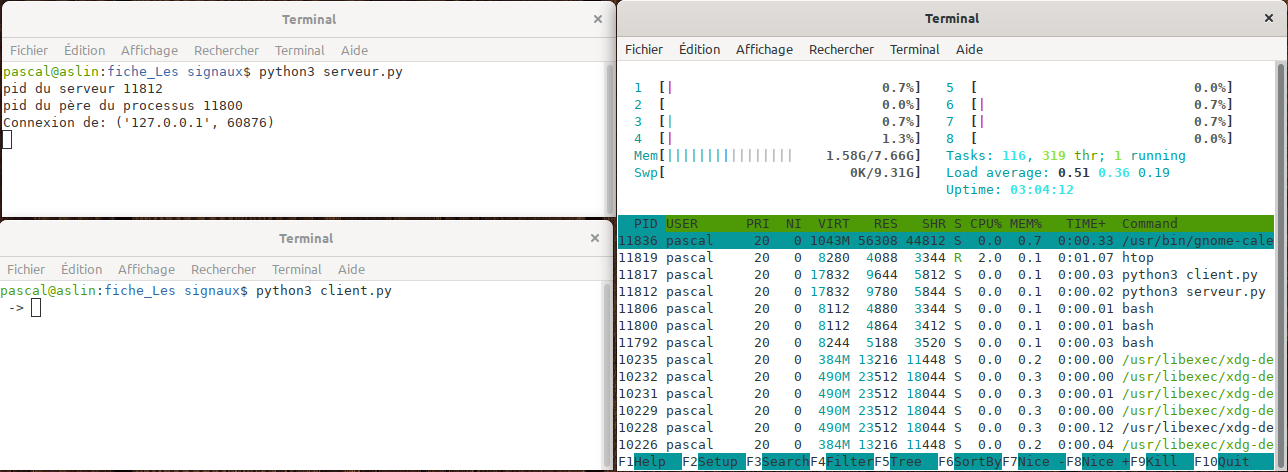
\includegraphics[width=0.5\linewidth]{bash_3x}
    \begin{enumerate}
        \item  Quel est le numéro pid du processus lié à  l'exécution de client.py ?    
        \item Quel(s) pourrait(aient) être le pid du parent du processus à  l'exécution de client.py ?
        \item Comment mettre fin au  processus associé serveur.py ? (donnez deux possibilités)       
    \end{enumerate}
    \item Tuez le serveur et continuez à envoyer des messages par le biais du client. Quelle message d'erreur apparaît? En expliquer la raison.
    Aurait-on pu procéder différemment ?
    \item Modifier le programme client pour que le programme prenne en considération cette erreur en demandant à l'utilisateur s'il veut continuer ou s'il veut mettre fin au programme.
\end{enumerate}
\end{exercise}

\end{frame}
%-------------------------------- FRAME ---------------------------------------------------
\begin{frame}{Corrigé exercice : question 2}
    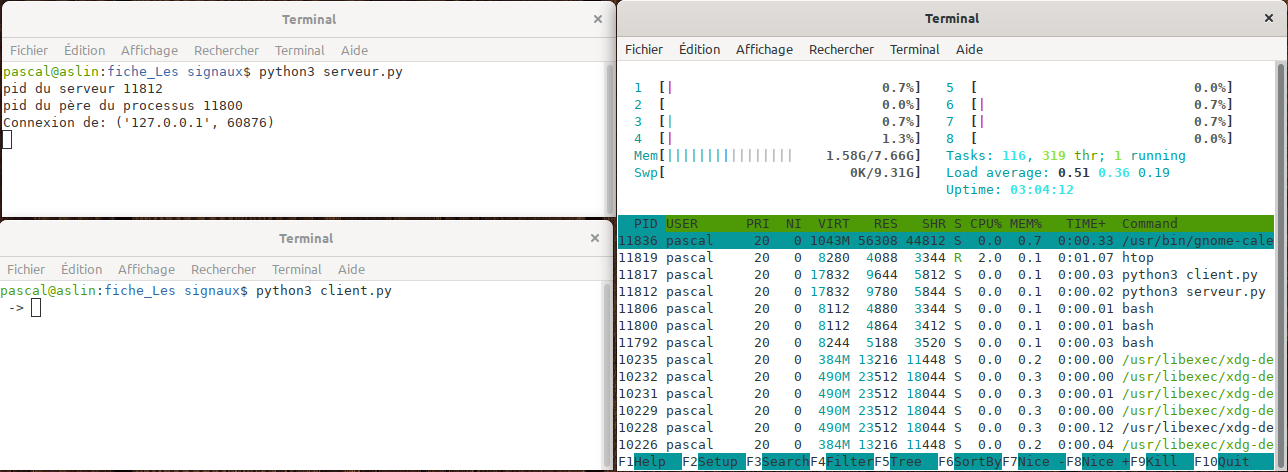
\includegraphics[width=1\linewidth]{bash_3x}
\begin{enumerate}
    \item[]
    \setcounter{enumi}{2}
   \begin{enumerate}[<+->]
  \item  Quel est le numéro pid du processus lié à  l'exécution de client.py ?
    \textbf{La commande \textit{ htop}  nous indique que le pid du client.py est 11817.}
    \item Quel(s) pourrait(aient) être le pid du parent du processus à  l'exécution de client.py ?\pause
    \textbf{Le parent est un programme \textit{bash}, donc en utilisant les informations de  \textit{htop} on voit qu'il peut s'agir du pid 11806 ou 11792}
    \item Comment mettre fin au  processus associé serveur.py ? (donnez deux possibilités)\pause
\textbf{En tapant Ctrl-C, avec  la fenêtre du terminal correspondant actif, en cliquant sur la croix de la fenêtre appropriée ou en tapant dans une console kill -2 11812.}
\end{enumerate}
\end{enumerate}
\end{frame}
%-------------------------------- FRAME ---------------------------------------------------
\begin{frame}{Corrigé exercice : question 3 }
\begin{enumerate}
    \setcounter{enumi}{2}
  \item Tuez le serveur et continuez à envoyer des messages par le biais du client. Quelle message d'erreur apparaît? En expliquer la raison.
 Aurait-on pu procéder différemment ?\pause
   \begin{itemize}[<+->]
     \item  \textbf{On a l'erreur suivante : BrokenPipeError: [Errno 32] Broken pipe.\\ En fermant le serveur, le canal de communication n'est plus disponible rendant impossible l'écriture des données dans le PIPE (canal, tuyau). Le programme client a reçu un signal SIGPIPE.}
     \item  \textbf{Il n'est pas nécessaire d'arrêter le serveur pour casser le canal de communication, on peut également exécuter la commande : } 
     kill -13 pid  (où pid est le numéro du processus à l'exécution du client).
 \end{itemize}

\end{enumerate}
\end{frame}
%-------------------------------- FRAME ---------------------------------------------------
\begin{frame}{Corrigé exercice : question 4}
 \only<1>{\begin{enumerate}[<+->]
    \setcounter{enumi}{3}
 \item 
Modifier le programme client pour que le programme prenne en considération cette erreur en demandant à l'utilisateur s'il veut continuer ou s'il veut mettre fin au programme.
\end{enumerate}
}
 \only<2>{
    \begin{code}{client.py}
        \inputminted[fontsize=\scriptsize]{Python}{client_cor.py}
    \end{code}
}
\end{frame}
\section*{Annexe}

\subsection{Description du fonctionnement CTRL-Z}
%-------------------------------- FRAME ---------------------------------------------------
\defverbatim[colored]\exii{
    \begin{minted}[autogobble, linenos]{Python}
    import signal
    import time
    
    def mongestionnaire(signum, stack):
    print('Alarme :', time.ctime())
    
    signal.signal(signal.SIGALRM, mongestionnaire)
    signal.alarm(2)
    
    print('Before:', time.ctime())
    time.sleep(4)
    print('After :', time.ctime())
    \end{minted}
}

\begin{frame}{Description du fonctionnement CTRL-Z}
Dans le terminal 
% Nécessite le package tikz
\begin{center}
    \begin{tikzpicture}[
    f/.style={->,very thick,>=stealth'},%
    s/.style={draw,circle},%
    p/.style={fill=white,inner sep=3pt},scale=0.8]
    \node[fill=pink,inner sep=10pt] (T1) at (0,0) {shell} ;
    \node[s,fill=yellow] (Cat) at (-2,-3) {Proc 1} ;
    \draw(-2,-4)node{\footnotesize pid:5341};
    \node[s,fill=blue!8] (FG) at (3,-3) {Proc 2} ;
    \draw[f] (T1) -- (Cat) node[pos=0.5,p]{$cat$} ;
    \draw[dashed](-3,-2)rectangle(-1,-5)node(fg)[below]{travail de premier plan};
    \draw[dashed](2,-2)rectangle(4,-5)node[below]{travail d'arrière plan};
    \draw[f] (T1) -- (FG) node[pos=0.5,p]{$Cmd \&$} ;
    %\draw(4,-7)node[text width=5cm](sign){Les signaux Ctrl-C et Ctrl-Z s'adressent à ce(s)  travail(aux)};
    %\draw[->](sign.west) to [out=180,in=270](fg.south);
    \end{tikzpicture}
\end{center}
\pause
La commande \textbf{Ctrl-Z } va passer le processus \textbf{cat} dans les travaux en arrière plan et changer son état en \textbf{Stopped} .  On aurait pu également taper la commande \textbf{kill SIGSTP 5341 } (\textit{si 5341 est le pid du processus de cat}). L'état \textbf{Stopped} du processus \textbf{cat}  interdit au processus de s'exécuter. La reprise est assurée à la réception du signal SIGCONT.
\end{frame}

\begin{frame}{Description du fonctionnement CTRL-Z}
\begin{center}
    \begin{tikzpicture}[
    f/.style={->,very thick,>=stealth'},%
    s/.style={draw,circle},%
    p/.style={fill=white,inner sep=3pt},scale=0.8]
    \only<+->{
    \node[fill=pink,inner sep=10pt] (T1) at (0,0) {shell} ;
    \node[s,fill=yellow] (Proc) at (-2,-2.7) {ps} ;
    \node[s,] (FG) at (5,-3) {Proc 2} ;
    \node[s,fill=blue!8] (Cat) at (3,-3) {Proc 1} ;
    \draw(3,-4)node{\footnotesize pid:5341};

    
    \draw[f] (T1) to  (Proc) ;
    \draw[f] (T1) -- (Cat)  ;
    \draw[f] (T1) -- (FG) ;
    \draw[dashed](-3,-2)rectangle(-1,-5)node(fg)[below]{travail de premier plan};
    \draw[dashed](2,-2)rectangle(6,-5)node[below]{travail d'arrière plan};
}
    \only<+->{
            \node[s] (kill) at (-5,-1) {\small kill -2 5341} ;
        \draw[->](kill)--(-3,-3)node[midway,above,rotate=-45]{signal};
    }
    \only<+->{
    \draw(4,-6.5)node[text width=6.5cm](sign){Les signaux Ctrl-C et Ctrl-Z ne s'adressent qu'aux travaux de premier plan};
    \draw[->](sign.west) to [out=180,in=270](fg.south);
}
    
    \end{tikzpicture}
\end{center}
\pause

La commande \textbf{killall -2 cat } n'a pas d'action sur le processus \textbf{cat}  car il ne fait partie des processus qui sont au premier plan. 

\noindent À l'aide de la commande \textbf{bg} (signal SIGCONT) le processus réintègre les processus de premier plan.

\end{frame}
\begin{frame}{Description du fonctionnement CTRL-Z}
\begin{center}
    \begin{tikzpicture}[
    f/.style={->,very thick,>=stealth'},%
    s/.style={draw,circle},%
    p/.style={fill=white,inner sep=3pt},scale=0.8]
    \node[fill=pink,inner sep=10pt] (T1) at (0,0) {shell} ;
    % \node[s,fill=yellow] (Proc) at (-2,-2.7) {ps} ;
    \node[s,fill=blue!8] (FG) at (3,-3) {Proc 2} ;
    \node[s,forbidden sign,fill=yellow] (Cat) at (-2,-3) {Proc 1} ;
    \draw(-2,-4)node{\footnotesize pid:5341};
    \node[s] (kill) at (-5,-1) {\small kill -2 5341} ;
    \draw[red, ->,very thick](kill) to (Cat) ;
    
    % \draw[f] (T1) to  (Proc) ;
    \draw[f] (T1) -- (Cat)  ;
    \draw[f] (T1) -- (FG) ;
    \draw[dashed](-3,-2)rectangle(-1,-5)node(fg)[below]{travail de premier plan};
    \draw[dashed](2,-2)rectangle(4,-5)node[below]{travail d'arrière plan};
    \draw(4,-7)node[text width=6cm](sign){Le signal SIGINT (kill -2) peut être délivré au processus destinataire, qui va se terminer, puisqu'il s'agit de l'action par défaut.};
    \draw[->](sign.west) to [out=180,in=270](fg.south);
    
    \end{tikzpicture}
    
\end{center}
\end{frame}
\end{document}
